\begin{frame}
\frametitle{Задача Producer-а и Consumer-а}
\begin{itemize}
    \item<1->Рассмотрим следующую задачу:
    \begin{itemize}
        \item<2->Producer - поток/потоки, который генерирует данные;
        \item<3->Consumer - поток/потоки, который потребляет данные;
        \item<4->что если Producer и Consumer работают с разной скоростью?
    \end{itemize}
\end{itemize}
\end{frame}

\begin{frame}
\frametitle{Переменная состояния}
\begin{itemize}
    \item<1->Перемнная состояния (condition variable) - объект и несколько
         методов для работы с ним
    \begin{itemize}
        \item<2->wait - ожидает, пока кто-нибудь не просигналит;
        \item<3->notify\_one - просигналить одному из ожидающих;
        \item<4->notify\_all - просигналить всем ожидающим.
    \end{itemize}
\end{itemize}
\end{frame}

\begin{frame}[fragile]
\frametitle{Переменная состояния}
\begin{lstlisting}
    struct lock;
    void lock(struct lock *lock);
    void unlock(struct lock *lock);

    struct condition;
    void wait(struct condition *cv, struct lock *lock);
    void notify_one(struct condition *cv);
    void notify_all(struct condition *cv);
\end{lstlisting}
\end{frame}

\begin{frame}[fragile]
\frametitle{Producer}
\begin{lstlisting}
    struct condition cv;
    struct lock mtx;
    int value;
    bool valid_value;
    bool done;

    void produce(int x)
    {
        lock(&mtx);
        while (valid_value)
            wait(&cv, &mtx);
        value = x;
        valid_value = true;
        notify_one(&cv);
        unlock(&mtx);
    }

    void finish(void)
    {
        lock(&mtx);
        done = true;
        notify_all(&cv);
        unlock(&mtx);
    }
\end{lstlisting}
\end{frame}

\begin{frame}[fragile]
\frametitle{Consumer}
\begin{lstlisting}
    int consume(int *x)
    {
        int ret = 0;
        lock(&mtx);

        while (!valid_value && !done)
            wait(&cv, &mtx);

        if (valid_value) {
            *x = value;
            valid_value = false;
            notify_one(&cv);
            ret = 1;
        }
        unlock(&mtx);
        return ret;
    }
\end{lstlisting}
\end{frame}

\begin{frame}[fragile]
\frametitle{Зачем нам lock?}
\begin{columns}
    \begin{column}{.4\textwidth}
        \begin{lstlisting}


/* lock(&mtx); */
done = true;
notify_all(&cv);
/* unlock(&mtx); */



        \end{lstlisting}
    \end{column}
    \begin{column}{.4\textwidth}
        \begin{lstlisting}
/* lock(&mtx); */
while (... && !done)




    wait(&cv, &mtx);
...
/* unlock(&mtx); */
        \end{lstlisting}
    \end{column}
    \begin{column}{.2\textwidth}
    \end{column}
\end{columns}
\end{frame}

\begin{frame}
\frametitle{Зачем нам цикл?}
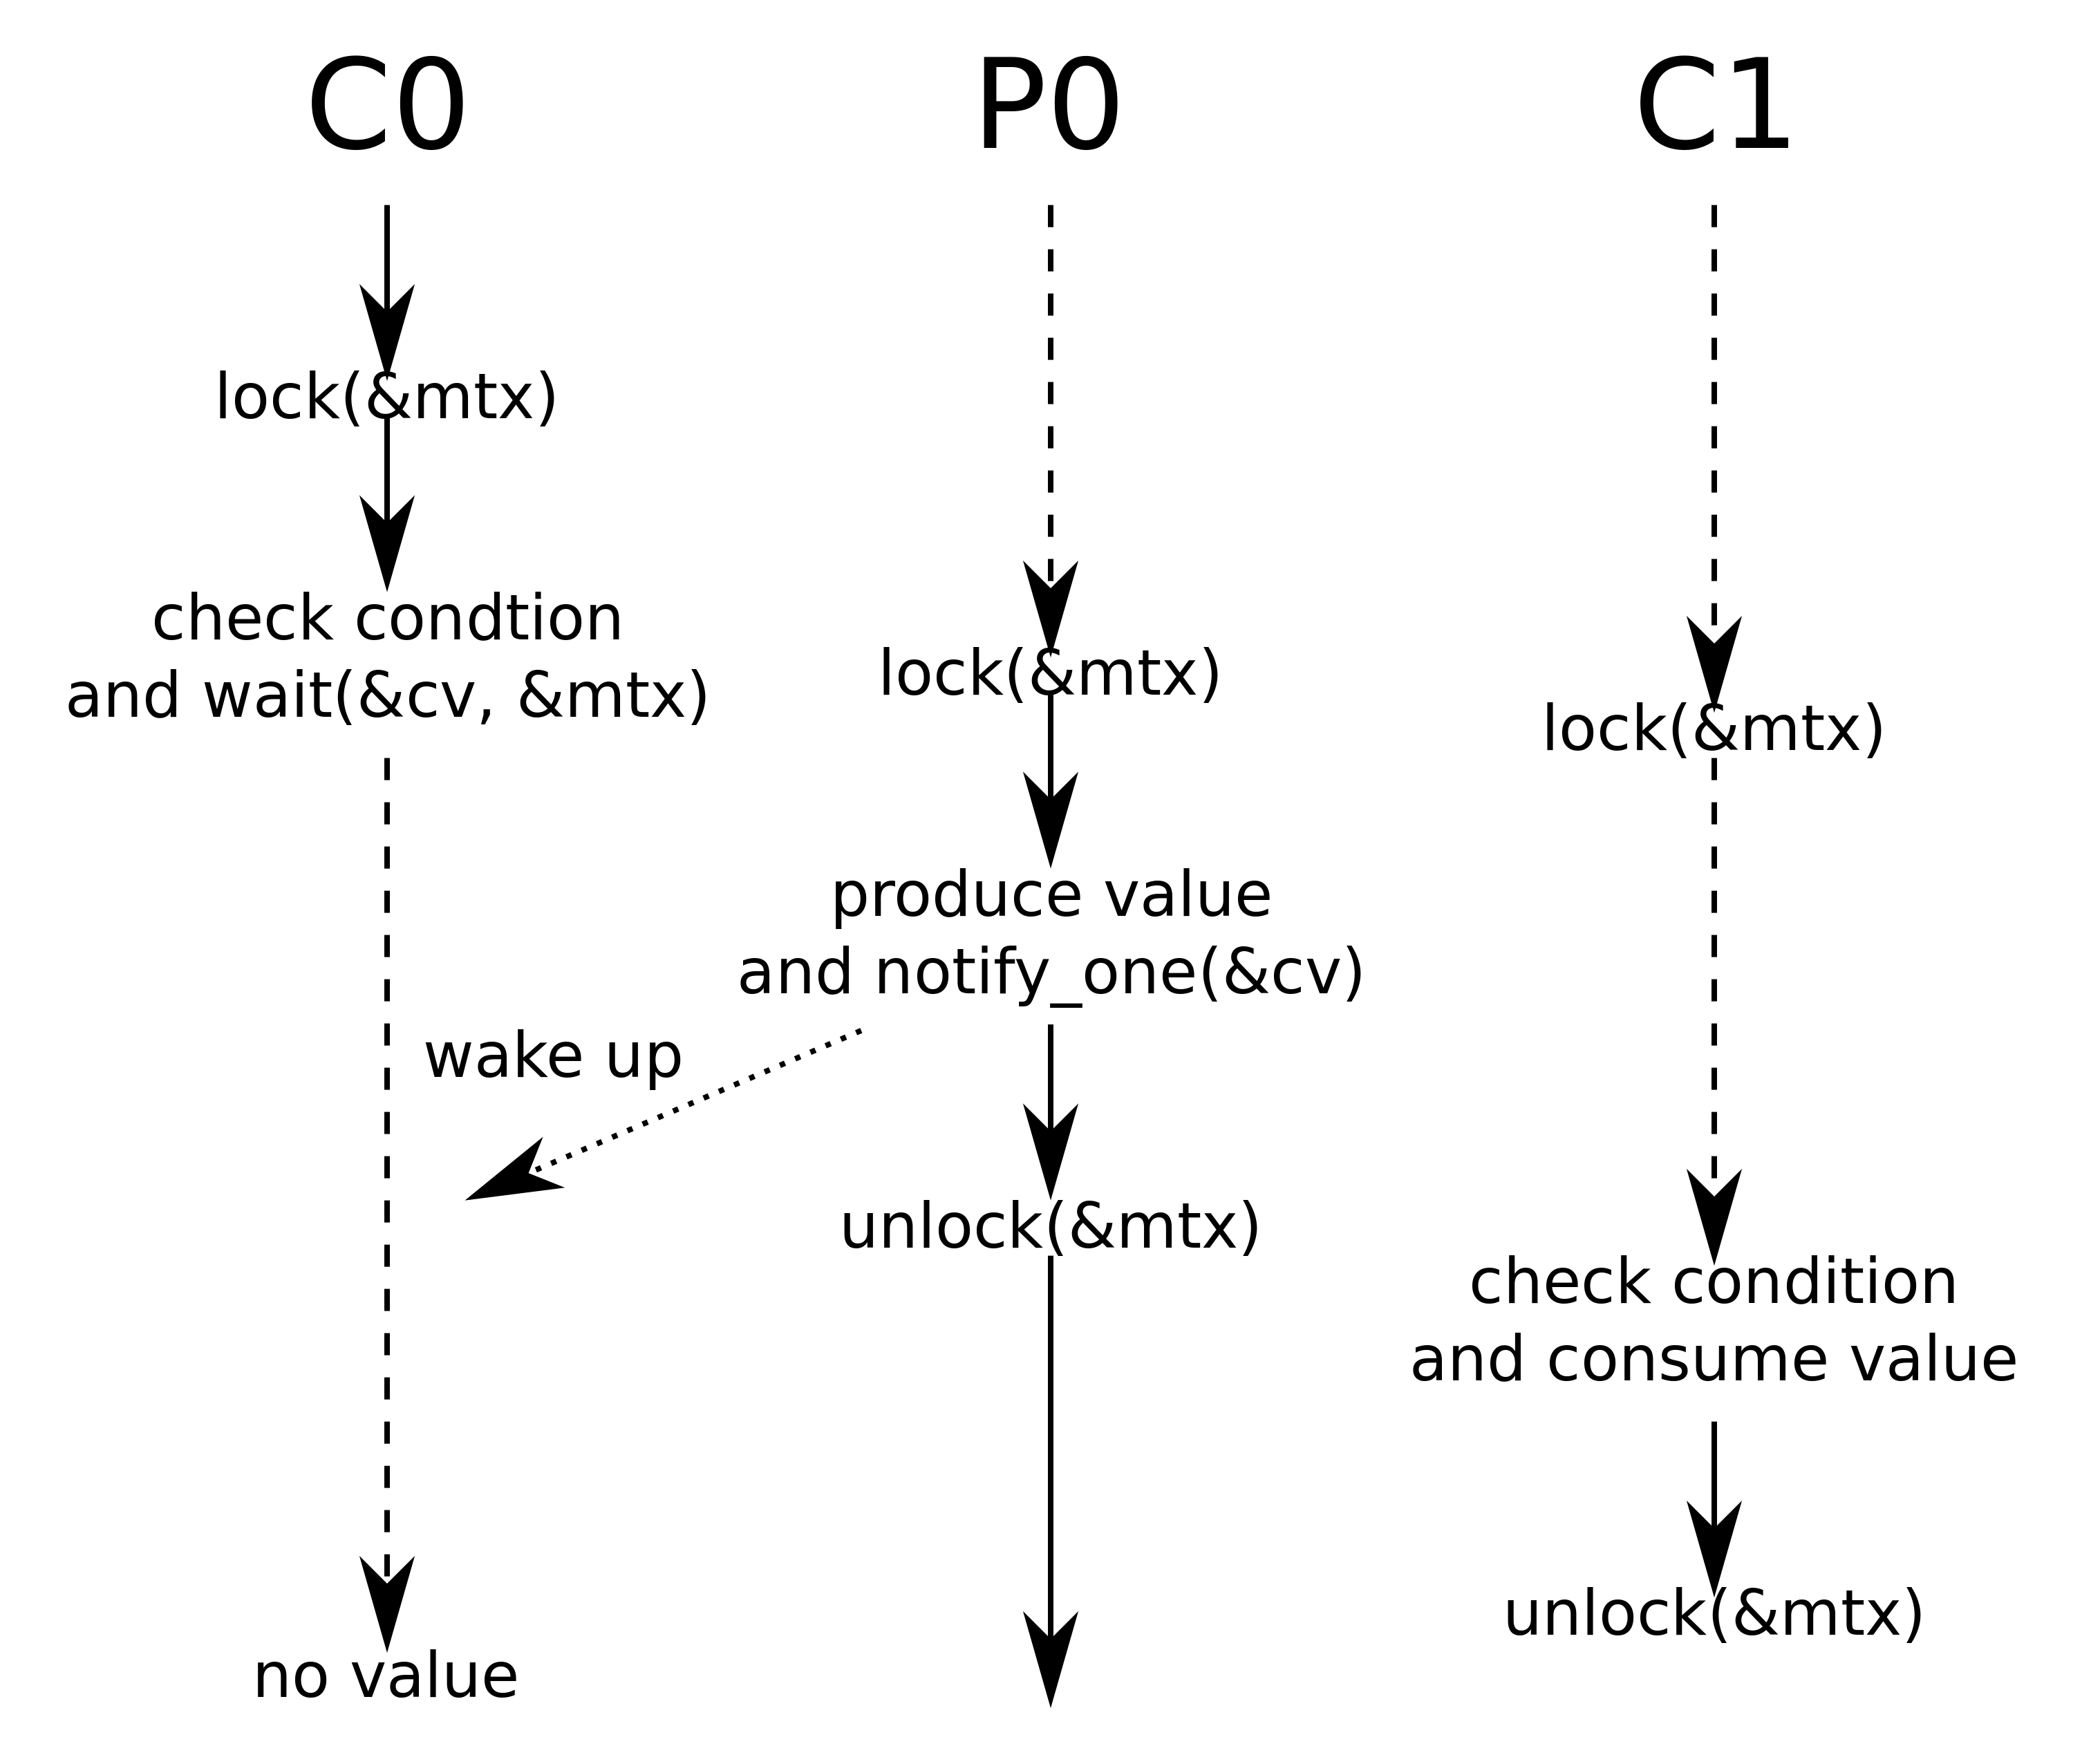
\includegraphics[height=.6\textheight]{cv}
\end{frame}

\begin{frame}
\frametitle{Зачем нам цикл?}
\begin{itemize}
    \item<1->Spurious wakeups (ложные пробуждения) - ситуация когда wait
         возвращает управление даже если никто не сигналил
    \begin{itemize}
        \item<2->многие реализации переменной состояния подвержены:
        \begin{itemize}
            \item<3->С++;
            \item<4->Java;
            \item<5->POSIX Threads...
        \end{itemize}
    \end{itemize}
\end{itemize}
\end{frame}
